%\documentclass[]{scrartcl}
\documentclass[]{article}
% sans-serif font
\renewcommand{\familydefault}{\sfdefault}

% Bibtex citations
%\usepackage{cite}
% sequence diagrams
\usepackage{pgf-umlsd}
% one inch margins
\usepackage[a4paper, margin=1in]{geometry}
% url referencing
\usepackage{url}
% show reference and figure lists in table of contents
\usepackage[nottoc,numbib]{tocbibind}
% add number to list of figures in table of contents
%\renewcommand{\listoffigures}{\begingroup
%\tocsection
%\tocfile{\listfigurename}{lof}
%\endgroup}

\usepackage{tikz,tkz-euclide}
% tikz features
\usetikzlibrary{decorations.pathreplacing,angles,quotes,shapes,arrows,fit}
\usetikzlibrary{calc} % coordinates
\usetikzlibrary{arrows.meta} % better arrows
\usetkzobj{all}

% real numbers symbol
\usepackage{amssymb}

% set default arrow
\tikzset{>=Latex}

% define arrow style
\tikzstyle{arw}=[-{Latex[length=3mm]}]

% extra math
\usepackage{mathtools}

% icons!
\usepackage{fontawesome}

% bigger dot for multiplication
\makeatletter
\newcommand*\bigcdot{\mathpalette\bigcdot@{.5}}
\newcommand*\bigcdot@[2]{\mathbin{\vcenter{\hbox{\scalebox{#2}{$\m@th#1\bullet$}}}}}
\makeatother

\title{Minecraft: Ray Traced}
%\subtitle{Or: A dynamic acceleration structure for voxel worlds}
\author{Marco Jonkers}

\begin{document}

%\maketitle

\begin{titlepage}
  \centering
  
\includegraphics[scale=0.5]{eng_logofc_uas.jpg}\par\vspace{1cm}
  {\scshape\LARGE NHTV Breda University of Applied Sciences\par}
  \vspace{1cm}
  {\scshape\Large Personal project\par}
  \vspace{1.5cm}
  {\huge\bfseries Minecraft: Ray Traced\par}
  \vspace{2cm}
  {\Large Marco Jonkers\par}
  \vspace{0.5cm}
  {Supervisor: David H{\"o}rchner\par}

  
  \vspace{2cm}
  
  \begin{abstract}
    This project attempts to implement a GPU ray tracer in the video game Minecraft, using CUDA.
    The ray tracing itself is done in CUDA. At first, I attempt to ray trace the vertex buffers given by Minecraft. Then, I implement my own data structures for increased performance.
  \end{abstract}
  
  \vfill
  
  % Bottom of the page
  {\large \today\par}
\end{titlepage}

% TODO: Do I want to keep the list of figures?

\newpage
\tableofcontents
%\listoffigures
\newpage

\section{Minecraft}
Minecraft is a 2011 first-person sandbox video game.
Originally created by Markus "Notch" Persson, it is currently maintained by Mojang.


Minecraft comes in multiple editions, for various platforms. This paper focuses on the PC version of Minecraft, released for Windows, macOS, and Linux.
The PC version is written in Java.

In Minecraft, the game world consists of a three-dimensional grid.
The world is procedurally generated, using a 
mostly comprised of unit blocks, as shown in Figure \ref{fig:ss-worldgen}.

\begin{figure}
  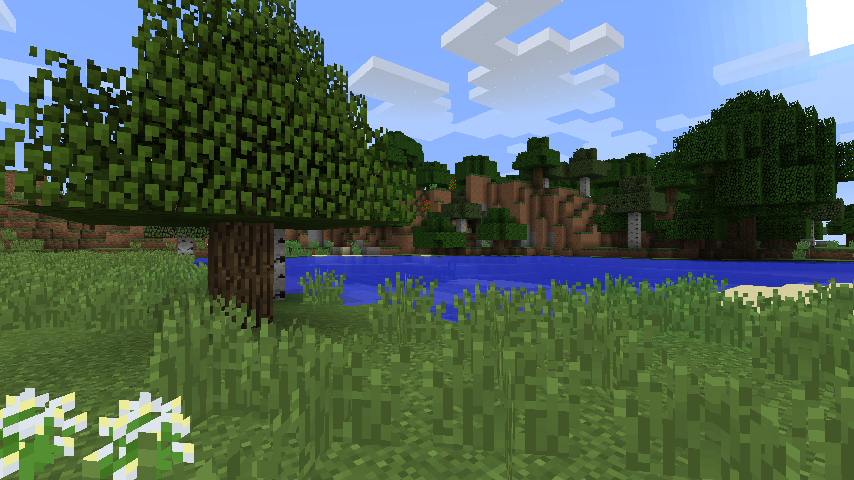
\includegraphics[width=\textwidth]{ss-worldgen.png}
  \centering
  \caption{In-game screenshot of Minecraft, without heads-up display (HUD) or viewmodel.}
  \label{fig:ss-worldgen}
\end{figure}

\section{Minecraft Renderer}
Minecraft uses multi-threaded chunk generation.
Minecraft uses OpenGL.
Minecraft has two options for rendering static geometry:
\begin{description}
  \item[Display Lists] An OpenGL 1.0 core function.
    Display Lists are a group of OpenGL commands that have been compiled and sent to the GPU.
    An object can then be drawn by calling the list.
    The list can be reused, which means you do not have to send the data over again.
  \item[Vertex Buffer Objects] Vertex Buffer Objects ("VBOs") were available in OpenGL 1.4 through an extension, and were later added to the core specification in version 2.1.
    This feature allows you to have a buffer with vertex information, and telling the driver where and how the attributes are stored in the buffer.
\end{description}
My project makes use of Minecraft's VBO rendering, because I can extract the vertex data from the buffers.
\subsection{RenderChunks}
There are four geometry groups, based on texture properties.
\begin{description}
  \item[Solid] Uses textures that are fully opaque. Most world blocks are in this group.
  \item[Cutout] Uses textures that have transparent texels.
  \item[Mipped Cutout] Identical to Cutout, but mipmapped.
  \item[Translucent] Used for block which have partial transparency (alpha blending).
\end{description}

\begin{figure}
  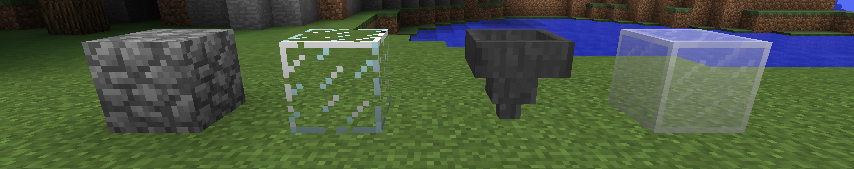
\includegraphics[width=\textwidth]{ss-layers.png}
  \centering
  \caption{From left to right: Cobblestone (Solid), Glass (Cutout), Hopper (Cutout Mipped), and Stained Glass (Translucent).}
  \label{fig:ss-layers}
\end{figure}
Every geometry group has its own vertex buffer.

\section{Minecraft Forge}
Minecraft Forge ("Forge") is a community created platform for developing and using modifications ("mods") for Minecraft.\footnote{Modification of Minecraft ("modding") is not officially supported by Mojang. For more information, visit \url{https://account.mojang.com/terms}}
\subsection{Setting up a mod development environment}
The Mod Development Kit ("MDK") can be downloaded from the Forge website\footnote{\url{http://files.minecraftforge.net/}}.
The MDK distribution includes ForgeGradle\footnote{\url{https://github.com/MinecraftForge/ForgeGradle}}.
ForgeGradle is a plugin for the Gradle\footnote{\url{https://gradle.org/}} build system.
The Minecraft binaries are downloaded, and subsequently decompiled, deobfuscated, 
The classes are decompiled into srg names.

The Mod Coder Pack\footnote{\url{http://www.modcoderpack.com/website/}} is a package which is used to decompile, change, and recompile Minecraft Java classes.

The Gradle tasks include:
\begin{enumerate}
  \item Download Minecraft .jar files.
  \item Decompile the Minecraft 
  \item Generate the Forge Minecraft binary
\end{enumerate}

Forge explicitly supports the Eclipse and IntelliJ integrated development environments ("IDEs").
I used IntelliJ IDEA Community.
ForgeGradle gives you the option of debugging and building both client and server sides of Minecraft.

The path to my DLLs is passed to the virtual machine.

\subsection{Differences between development and release builds}
During development, Java loads my classpath directly.
In release mode, my class files would have to be compressed into an archive first.

\subsection{Changes to Minecraft source code}
Forge adds some new features to the Minecraft source code, in order to support multi-mod functionality.

\subsection{Creating a mod}
In general there are three approaches to creating a mod:
\begin{enumerate}
  \item Build a mod on top of the Forge Minecraft code
  \item Edit the Minecraft source directly
  \item Use class transformers in custom mod loading
\end{enumerate}
For most mods, the first approach is sufficient.
This also enables the developer to freely distribute their mod.
Editing the Minecraft source directly means that the mod cannot be redistributed, because the original Minecraft code is copyrighted.


\section{C++ and CUDA}
I wanted to create a GPU ray tracer.
There are various methods to achieve this. 
I wanted to take advantage of the vertex buffers in CUDA.
Because Minecraft uses OpenGL through the LWJGL\footnote{\url{https://www.lwjgl.org/}} library, I could have chosen to use OpenGL compute shaders.
However, I have no experience with OpenGL compute shaders, whereas I do have experience with NVIDIA CUDA.

There exist Java bindings for CUDA, but using C++ removes my dependency on a binding layer.
\subsection{Java Native Interface}
Java Native Interface ("JNI") is a programming framework that allows for Java code to interact with native code.
\subsection{CUDA}
CUDA is a parallel computing platform and programming model developed by NVIDIA.
It is only compatible with NVIDIA hardware.
CUDA has two APIs: Runtime and Driver.
\subsection{CUDA/OpenGL interoperability}
CUDA provides an API for operating on OpenGL primitives.
\begin{enumerate}
  \item Run the ray tracing kernel
  \item Map the OpenGL texture to a CUDA array
  \item Copy the kernel output buffer to the CUDA array
\end{enumerate}

\subsection{Creating a Visual Studio project}
For setting up the native part of the mod, I created a Visual Studio CUDA project.
NVIDIA has a CUDA plugin for Visual Studio called Nsight.

\tikzstyle{dll}=[draw,rectangle,text width=2cm,text centered,node distance=3.5cm]
\tikzstyle{java}=[draw,rectangle,inner sep=0.3cm,rounded corners,node distance=3.5cm,minimum width=8em,minimum height=4em]
\begin{figure}
  \begin{tikzpicture}[auto]
  % loader.dll
  \node[dll] (loader_dll) {loader.dll};
  % raytracer.dll
  \node[dll,right of=loader_dll] (raytracer_dll) {raytracer.dll};
  % Raytracer.class
  \node[java,fit=(loader_dll)] (container) {};
  % Raytracer.class label
  \node at (container.north)[above](raytracer){Raytracer.class};
  % mcraytracer.jar
  \node[java,fit=(container)(raytracer)](minecraft){};
  % mcraytracer.jar label
  \node at (minecraft.north)[above](jar){mcraytracer.jar};
  % minecraft jar
  \node[java,left of=raytracer](minecraft_jar){minecraft.jar};
  % Forge Minecraft
  \node[java,below of=minecraft_jar](forge_minecraft){Forge Minecraft};
  \node[java,right of=forge_minecraft](external_libraries){External libraries};
  % Java Virtual Machine
  \node[java,fit=(jar)(minecraft)(minecraft_jar)(forge_minecraft)(external_libraries)](java){};
  % Java Virtual Machine label
  \node at (java.north)[above](vm_label){Java Virtual Machine};
  
  \draw [->] (loader_dll) -- node {} (raytracer_dll);
  %\draw [<->] (minecraft_jar) -- node {} (minecraft);
  \end{tikzpicture}
  \centering
  \caption[Binary interaction]{Interaction diagram of the different binaries.}
  \label{fig:modules}
\end{figure}

\subsubsection{Reloading C++}
Java IDEs such as IntelliJ support hot-swapping of method bodies by using the HotSwap functionality of the Java Platform Debugger Architecture.
I created something similar for my native code by using a technique called DLL reloading.
Once a native library has been loaded by the JVM, I cannot make changes to it.
Therefore I am using a passthrough DLL, which passes the calls from Java to another DLL.
I have shown this in Figure \ref{fig:modules}.

\subsubsection{Setting up the Visual Studio debugger}
IntelliJ debug sessions are good for testing if my Java ASM works correctly, and if my JNI bindings are set up properly.
However, if an error occurs a native part, the debug session ends immediately.
The crash output from IntelliJ is unable to use the debug information from Visual Studio.
I wanted to use the Visual Studio debugger for the native part.
I had to launch java.exe with the right command line arguments and working directory.
I looked at the launch parameters given to java.exe when starting a debug session from IntelliJ.
The Visual Studio debugger can be configured to launch Minecraft by copying the command line arguments from an IntelliJ debug session.
The JVM uses the access violation signal internally for its memory exception handling.
When an access violation is thrown from the JVM, this can be safely ignored.
However, Visual Studio can easily block hundreds of these signals.
Visual Studio 2017 offers an option to ignore certain exceptions per module, allowing me to break on access violations in my own native code while ignoring those coming from the JVM.

\subsection{Kernel overhead on Windows}

\section{Hardware}
This project is developed on the following machines:

\begin{center}
  \begin{tabular}{| l || c | c |} \hline
    & Dell XPS 15 L502X & Desktop \\ \hline
    Operating System & \multicolumn{2}{c|}{Microsoft Windows 10 Pro 64-bit} \\ \hline
    Processor & Intel Core i7-2630QM & Intel Core i7-4790 \\ \hline
    Memory & 4 GB DDR3 & 8 GB DDR3 \\ \hline \hline
    GPU & NVIDIA GeForce GT 540M & NVIDIA GeForce GTX 970\\ \hline
    - CUDA Cores & 96 & 1664 \\ \hline
    - Shader Multiprocessors & 2 & 13 \\ \hline
    - Compute Capability & 2.1 & 5.2 \\ \hline
    %- Processor Clock & 1344 MHz &  \\ \hline
    - Memory Clock & 900 MHz & 7010 MHz \\ \hline
    - Graphics Clock & 672 MHz & 1140 MHz \\ \hline
    - Memory & 2 GB & 4 GB\footnote{\url{https://blogs.nvidia.com/blog/2015/02/24/gtx-970/}}\\ \hline
  \end{tabular}
\end{center}

\begin{equation}
  f(s, ds) =
  \begin{cases}
    \frac{\lceil s \rceil - s}{\lvert ds \rvert} & ds > 0 \\
    \frac{s - \lfloor s \rfloor}{\lvert ds \rvert} & ds < 0 \\
    \infty & ds = 0
  \end{cases}
\end{equation}

\section{Ray Tracing OpenGL Vertex Buffers}
My initial idea was to ray trace the uploaded VBOs from Minecraft directly.


\subsection{Forge Events}
I wanted to see if I could make my mod work using the first approach.
Forge adds hooks to the game loop which I could use to intercept the rendering code.
The \texttt{Raytracer} class listens to the following events:
\begin{itemize}
  \item \texttt{FMLInitializationEvent} \\
    As the name indicates, this event is fired when Forge is initializing Minecraft.
    This event is used to initialize the mod.
    Here I also obtain a reference to the \texttt{Minecraft} singleton class.
    The mod needs to be registered in the \texttt{ClientRegistry} in order to receive further Forge events.
  \item \texttt{TickEvent.ClientTickEvent} \\
    This event is fired 20 times per second, and can be regarded as the client-sided update function.
    I listen to this event to check for keyboard input changes.
  \item \texttt{GuiScreenEvent.InitGuiEvent.Pre} \\
    This is the first event that is fired when a window resize is detected.
    The event does not contain any resize information, so I track it manually.
    The resolution information in the \texttt{Minecraft} class is public, so I extract it from there.
    The information is passed to C++, such that the CUDA and OpenGL resources can be resized if they need to be.
    OpenGL supports resizing by calling \texttt{glTexImage2D} with the new information, without having to call \texttt{glGenTextures} again.
    In CUDA, it is required to unregister and re-register the associated graphics resource.
    The kernel output buffer is also resized. This uses a pair of \texttt{cudaFree} and \texttt{cudaMalloc} calls.

    % TODO: something about OpenGL textures and power of two?
  \item \texttt{TickEvent.RenderTickEvent} \\
    This event is fired when Minecraft starts rendering the next frame.
    
    In order to prevent Minecraft from drawing the world after I have done the ray tracing, I copy the \texttt{WorldClient} reference from \texttt{Minecraft}, and set the value in \texttt{Minecraft} to \texttt{null}.
    This effectively causes Minecraft to skip the rendering of the game world, because it has an internal check for the \texttt{WorldClient} there.
    If it is \texttt{null}, nothing is rendered.
    However, this also disables rendering of the game overlay, which contains elements like the player inventory and menu's.
    I manually draw the game overlay after drawing the ray tracing result to the screen.
  \item \texttt{GuiScreenEvent.DrawScreenEvent.Pre} \& \texttt{GuiScreenEvent.DrawScreenEvent.Post} \\
    I noticed that the background of the game overlay was solid instead of transparent.
    This is due to another check for the \texttt{WorldClient} instance during drawing.
    Because I previously made it \texttt{null}, I now have to restore it on the \texttt{GuiScreenEvent.DrawScreenEvent.Pre} event in order to draw the background.
    I set it back to null at the \texttt{GuiScreenEvent.DrawScreenEvent.Post} event.
  %\item \texttt{GuiOpenEvent} \\
    %Fired when the top-level menu changes.
\end{itemize}

\subsection{Using Java ASM}

\subsection{C++/CUDA}
\texttt{cudaGraphicsGLRegisterBuffer}

\subsection{Results}



\section{Preprocessing Vertex Buffers}

\subsection{Obtaining the buffers}
In order to get the raw vertex buffers from Java to C++, I had to change three Minecraft classes.
My approach was to replace the built-in \texttt{VertexBuffer} class with my own class, called \texttt{CppVertexBuffer}.
Confusingly, the decompiled version of Minecraft has two classes called VertexBuffer in two separate packages.


\begin{description}
  \item[RenderChunk]
    The class that represents a 16x16x16 chunk of blocks.
    It contains one OpenGL vertex buffer per render layer.
  \item[ChunkRenderDispatcher]
  \item[VertexBufferUploader]
\end{description}

\subsection{Acceleration structure}

\section{Future work}
I only got to work on the world rendering of the game.
Viewmodels (player-held items) are not ray traced.
Non-playable characters ("NPCs") are not ray traced.

\bibliography{minecraft_ray_traced}{}
\bibliographystyle{plain}
%\bibliographystyle{apalike}

% Code flow structure
\begin{figure}
  \centering
  \label{fig:sequence}
  \begin{sequencediagram}
    \newthread{minecraft}{Forge Minecraft}{}
    \newinst[2]{forge}{Forge Mod}{}
    \newinst[2]{loader}{C++/CUDA}{}
    \begin{call}{minecraft}{transform()}{forge}{}
    \end{call}
    \postlevel
    \begin{call}{minecraft}{Raytracer()}{forge}{}
      \begin{call}{forge}{init()}{loader}{}
      \end{call}
    \end{call}
    %    \postlevel
    %    \begin{call}{minecraft}{onPreInitGuiEvent()}{forge}{}
    %      \begin{call}{forge}{resize()}{loader}{}
    %      \end{call}
    %    \end{call}
    \begin{sdblock}{Main Loop}{}
      \begin{call}{minecraft}{initialize()}{forge}{}
        \begin{call}{forge}{setViewEntity()}{loader}{}
        \end{call}
      \end{call}
      \postlevel
      \begin{call}{minecraft}{addRenderChunk()}{forge}{}
      \end{call}
      \postlevel
      \begin{call}{minecraft}{renderChunkLayer()}{forge}{}
        \begin{call}{forge}{setVertexBuffer()}{loader}{}
          \begin{call}{loader}{GetIntField()}{loader}{glBufferId}
          \end{call}
        \end{call}
      \end{call}
      \postlevel
      \begin{call}{minecraft}{renderWorld()}{forge}{}
        \begin{call}{forge}{setViewingPlane()}{loader}{}
        \end{call}
        \postlevel
        \begin{call}{forge}{raytrace()}{loader}{texture ID}
          \begin{call}{loader}{Kernel()}{loader}{}
          \end{call}
        \end{call}
      \end{call}
    \end{sdblock}
  \end{sequencediagram}
  \caption[Sequence diagram]{Sequence diagram showing interaction between the modules}
\end{figure}

% hfov = 102.4478577779882556443232935315
% ++(141.22392888899412782216164676575:6cm);
% ++(38.77607111100587217783835323425:6cm);

\begin{figure}
  \centering
  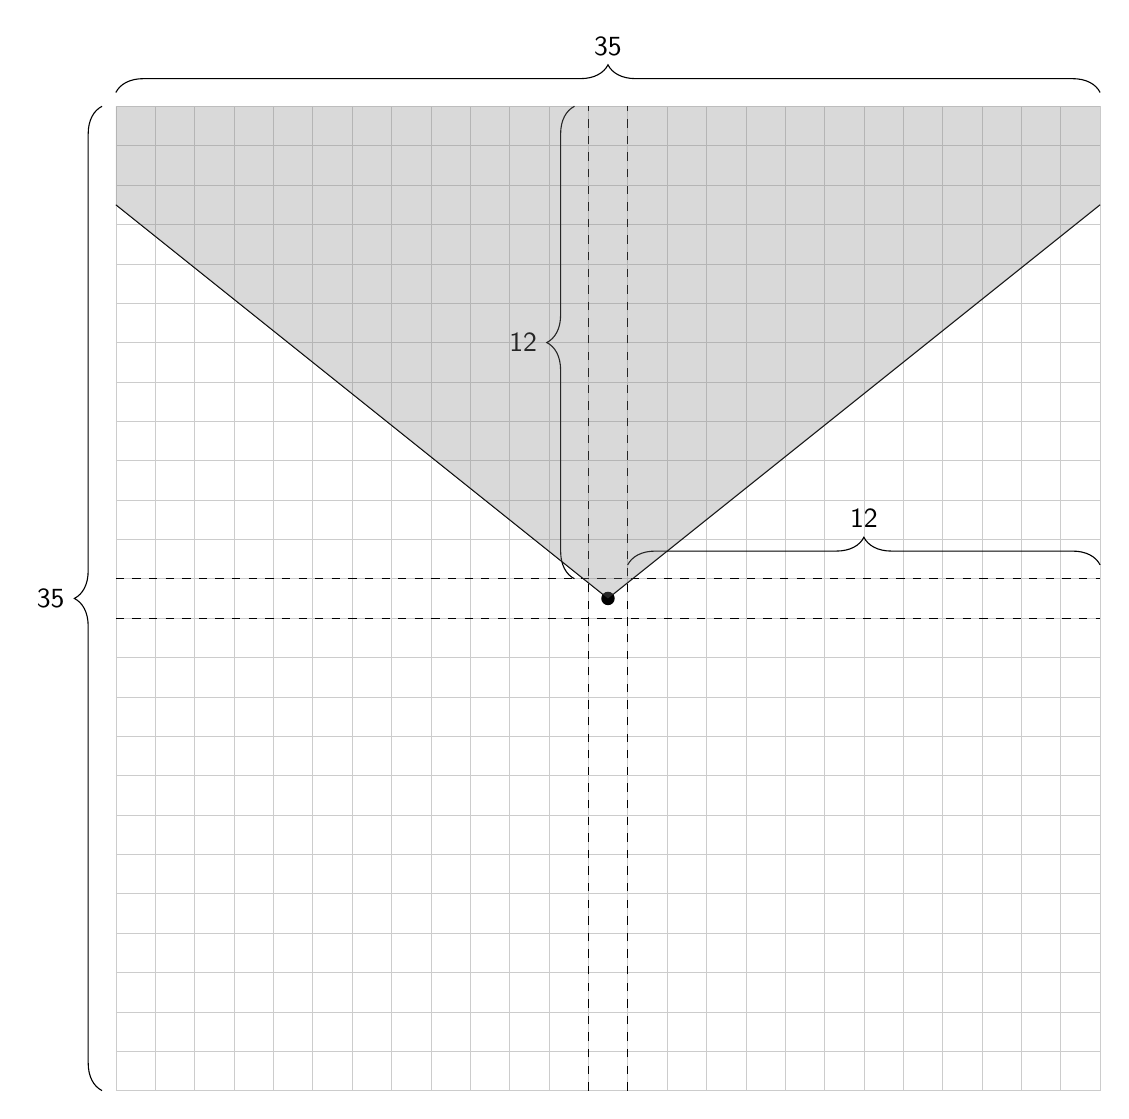
\begin{tikzpicture}
  \draw[step=0.5cm,very thin,opacity=0.2] (-6,-6) grid (6.5,6.5);
  %\fill (0,0) -- (0.5,0) -- (0.5,0.5) -- (0,0.5) -- (0,0);
  \draw[dashed] (-6,0) -- (6.5,0);
  \draw[dashed] (-6,0.5) -- (6.5,0.5);
  \draw[dashed] (0,-6) -- (0,6.5);
  \draw[dashed] (0.5,-6) -- (0.5,6.5);
  \draw[decoration={brace,amplitude=10pt,raise=5pt},decorate] (0.5,0.5) -- node[above=15pt] {12} (6.5,0.5);
  \draw[decoration={brace,amplitude=10pt,raise=5pt},decorate] (0,0.5) -- node[left=15pt] {12} (0,6.5);
  \draw[decoration={brace,amplitude=10pt,raise=5pt},decorate] (-6,6.5) -- node[above=15pt] {35} (6.5,6.5);
  \draw[decoration={brace,amplitude=10pt,raise=5pt},decorate] (-6,-6) -- node[left=15pt] {35} (-6,6.5);
  \draw[fill] (0.25,0.25) circle (.5ex);
  
  % view frustum
  \draw (0.25,0.25) -- (-6,5.25);
  \draw (0.25,0.25) -- (6.5,5.25);
  \fill[color=gray,opacity=0.3] (-6,6.5) -- (-6,5.25) -- (0.25,0.25) -- (6.5,5.25) -- (6.5,6.5);
  
  %\draw[decoration={brace,mirror,raise=5pt},decorate] (0.5,0) -- node[below=6pt] {Render distance} (6.5,0);
  \end{tikzpicture}
  \caption[Top-down view of vertex buffer array]{
    A top-down view of the vertex buffer array, assuming a render distance of 12.
    The player's view cone is shown facing north.
    Each cell contains 16 RenderChunks.
    When the player crosses a horizontal chunk boundary, every buffer in the grid is moved once space.
  }
  \label{fig:grid}
\end{figure}

\begin{figure}
  \centering
  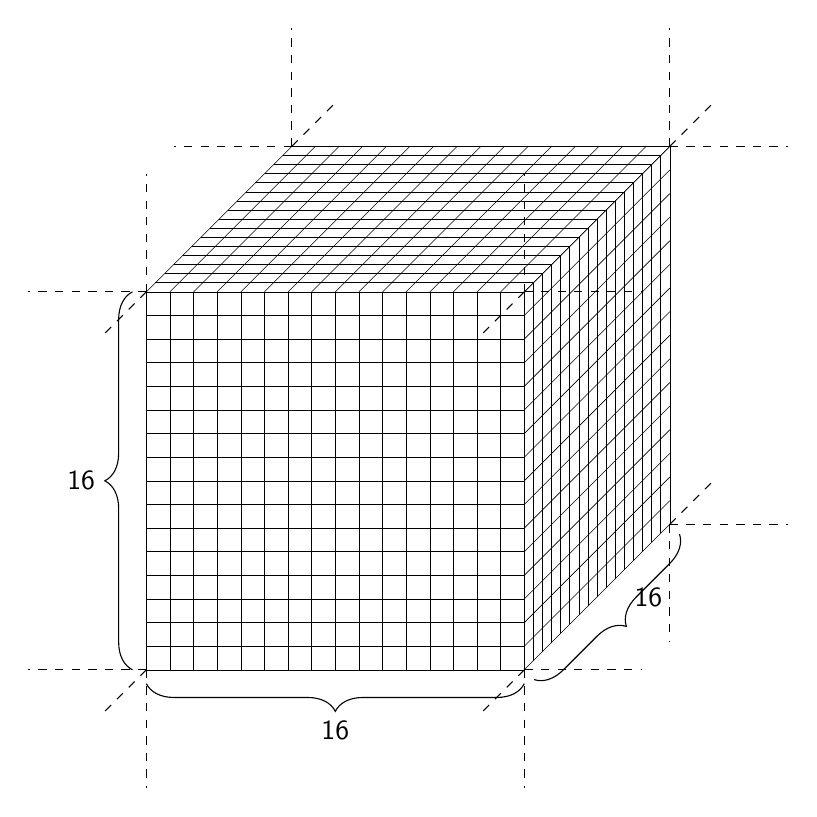
\begin{tikzpicture}[scale=0.3]
  \foreach \x in{0,...,16} {
    \draw[very thin] (0,\x ,16) -- (16,\x ,16);
    \draw[very thin] (\x ,0,16) -- (\x ,16,16);
    \draw[very thin] (16,\x ,16) -- (16,\x ,0);
    \draw[very thin] (\x ,16,16) -- (\x ,16,0);
    \draw[very thin] (16,0,\x ) -- (16,16,\x );
    \draw[very thin] (0,16,\x ) -- (16,16,\x );
  }
  % right
  \draw[dashed] (16,0,0) -- ++(5,0,0);
  \draw[dashed] (16,16,0) -- ++(5,0,0);
  \draw[dashed] (16,16,16) -- ++(5,0,0);
  \draw[dashed] (16,0,16) -- ++(5,0,0);
  % top
  \draw[dashed] (0,16,0) -- ++(0,5,0);
  \draw[dashed] (16,16,0) -- ++(0,5,0);
  \draw[dashed] (16,16,16) -- ++(0,5,0);
  \draw[dashed] (0,16,16) -- ++(0,5,0);
  % back
  \draw[dashed] (0,16,0) -- ++(0,0,-5);
  \draw[dashed] (16,16,0) -- ++(0,0,-5);
  \draw[dashed] (16,0,0) -- ++(0,0,-5);
  % front
  \draw[dashed] (0,16,16) -- ++(0,0,5);
  \draw[dashed] (16,16,16) -- ++(0,0,5);
  \draw[dashed] (16,0,16) -- ++(0,0,5);
  \draw[dashed] (0,0,16) -- ++(0,0,5);
  % left
  \draw[dashed] (0,0,16) -- ++(-5,0,0);
  \draw[dashed] (0,16,16) -- ++(-5,0,0);
  \draw[dashed] (0,16,0) -- ++(-5,0,0);
  % bottom
  \draw[dashed] (16,0,0) -- ++(0,-5,0);
  \draw[dashed] (16,0,16) -- ++(0,-5,0);
  \draw[dashed] (0,0,16) -- ++(0,-5,0);
  % curly braces
  \draw[decoration={brace,amplitude=10pt,raise=5pt},decorate] (0,0,16) -- node[left=15pt]{16} (0,16,16);
  \draw[decoration={brace,mirror,amplitude=10pt,raise=5pt},decorate] (0,0,16) -- node[below=15pt]{16} (16,0,16);
  \draw[decoration={brace,mirror,amplitude=10pt,raise=5pt},decorate] (16,0,16) -- node[below=15pt,right=10pt]{16} (16,0,0);
  \end{tikzpicture}
  \caption[Diagram of a RenderChunk]{A single, completely filled RenderChunk.}
\end{figure}

% TODO Rotate this diagram 90 degrees along Y axis
\begin{figure}
  \centering
  \begin{tikzpicture}[scale=0.5]
    \coordinate (A) at (0,0,0);
    \coordinate (B) at (0,0,16);
    \coordinate (C) at (0,9,0);
    \coordinate (D) at (0,9,16);
    \coordinate (E) at (0,4.5,8);
    \coordinate (F) at (-8,4.5,8);
    \coordinate (G) at (0,4.5,0);
    \coordinate (H) at (0,9,8);
    \coordinate (I) at (-5,0,0);
    \draw[arw] (A) node[anchor=north]{$P$} -- (B) node[anchor=north]{$Q$};
    \draw[arw] (A) -- (C) node[anchor=south]{$R$};
    \draw[dotted] (H) -- (E);
    \draw[dashed] (B) -- (D);
    \draw[dashed] (C) -- (D);
    \tkzMarkRightAngle[draw=black,size=0.5](H,E,F)
    \tkzMarkRightAngle[draw=black,size=0.5](C,A,I)
    \tkzMarkRightAngle[draw=black,size=0.5](C,G,E)
    \tkzMarkSegment[pos=.75,mark=|](A,C)
    \tkzMarkSegment[pos=.25,mark=|](A,C)
    
    % eye point stuff
    \draw[dotted] (E) node[anchor=north west]{$S$} -- (F) node[anchor=north]{\faVideoCamera};
    \draw[arw] (A) -- node[anchor=north west]{$\vec{u}$} (I);
    \draw[dotted] (H) -- (F);
    \draw[dotted] (G) -- (E);
    \pic [draw, -, "$\theta$", angle eccentricity=1.5] {angle = E--F--H};
  \end{tikzpicture}
  
  \begin{align}
  \theta& = \frac{vertical\ field\ of\ view}{2} \nonumber \\
  \vec{u}& = \overrightarrow{PQ}\times\overrightarrow{PR} \nonumber \\
  S& = \frac{Q + R}{2} \nonumber \\
  \text{\faVideoCamera}_{pos}& = S + \frac{\vec{u}}{\lvert\lvert\vec{u}\rvert\rvert}\bigcdot\frac{\lvert\lvert\overrightarrow{PR}\rvert\rvert}{2 \tan\left(\theta\right)} \label{eq:1}
  \end{align}
  \caption{Ray origin calculations}
\end{figure}

% TODO: Java class diagrams(minecraft, raytracer)

\end{document}
